\scanpage{11}

On trouve donc
\[
\boxed{L_E\left(\deleted{\unsure{t^{-1}}}\frac{1}{tp^{\rho}}\right)=\deleted{\unsure{(-t)^n}}\det f_E(-t)^nL_E(t)}
\]
[$\rho$ étant le poids de $E$, qui s'introduit via $\check E\simeq E(\rho)$]

\figure{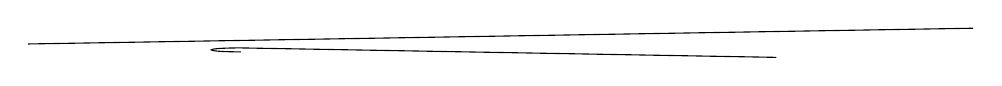
\begin{tikzpicture}[x=1cm,y=1cm]
\draw (0,0.25) -- (12,0.45);
\draw (2.7,0.15) .. controls (2.2,0.15) and (2.2,0.2) .. (2.7,0.2) -- (9.5,0.08);
\end{tikzpicture}}

Soit $E$ un $\mathbb{Q}_{\ell}$-faisceau constructible sur $X$ \deleted{compactifiable} \inserted{propre} sur $\mathbb{F}_p$, alors on aura
\deleted{
\[
H_c^i(X,DE)\simeq D(H^{-i}(X,E))
\]
}
par le th. de dualité globale
\deleted{d'où donc
\[
\chi(DE)=\sum(-1)^iH^i(X,D(E))\simeq D(\chi(E))
\]
}
\[
\mathbf{R}f_*(DE)=D(\mathbf{R}f_*(E))
\]
d'où
\[
\left\{\begin{aligned}
&\text{(1)}\quad\boxed{L_{DE}(t)=(-t)^{-\chi(E)}\delta(E)\,L_E(t^{-1})}\\
&\chi(E)=\operatorname{rang}\mathbf{R}f_*E=\sum(-1)^i\operatorname{rg}H^i(\bar X,\bar E)\\
&\delta(E)=\prod_i\left(\det f_{H^i(\bar X,\unsure{\bar F|\bar E})}\right)^{(-1)^i}=\varepsilon(E)p^{\sum_i(-1)^i\deleted{\unsure{\rho}}\frac{i+\rho}{2}b_i}
\end{aligned}\right.
\]
\inserted{avec les conjectures \unsure{standart|standard}, si $X$ est \deleted{\unsure{projectif|propre}} \inserted{lisse purement de dim $n$} \deleted{lisse} et $F$ \unsure{c$^{\mathrm{t}}$|c.t.} tordu \unsure{purement} de poids $\rho$}
\margin{invariant géométrique}
\margin{invariant arithmétique}
\margin{$b_i=\operatorname{rang}H^i(\bar X,\bar F)$}

\mspage{10}
